% Options for packages loaded elsewhere
\PassOptionsToPackage{unicode}{hyperref}
\PassOptionsToPackage{hyphens}{url}
%
\documentclass[
]{article}
\usepackage{amsmath,amssymb}
\usepackage{iftex}
\ifPDFTeX
  \usepackage[T1]{fontenc}
  \usepackage[utf8]{inputenc}
  \usepackage{textcomp} % provide euro and other symbols
\else % if luatex or xetex
  \usepackage{unicode-math} % this also loads fontspec
  \defaultfontfeatures{Scale=MatchLowercase}
  \defaultfontfeatures[\rmfamily]{Ligatures=TeX,Scale=1}
\fi
\usepackage{lmodern}
\ifPDFTeX\else
  % xetex/luatex font selection
\fi
% Use upquote if available, for straight quotes in verbatim environments
\IfFileExists{upquote.sty}{\usepackage{upquote}}{}
\IfFileExists{microtype.sty}{% use microtype if available
  \usepackage[]{microtype}
  \UseMicrotypeSet[protrusion]{basicmath} % disable protrusion for tt fonts
}{}
\makeatletter
\@ifundefined{KOMAClassName}{% if non-KOMA class
  \IfFileExists{parskip.sty}{%
    \usepackage{parskip}
  }{% else
    \setlength{\parindent}{0pt}
    \setlength{\parskip}{6pt plus 2pt minus 1pt}}
}{% if KOMA class
  \KOMAoptions{parskip=half}}
\makeatother
\usepackage{xcolor}
\usepackage[margin=1in]{geometry}
\usepackage{color}
\usepackage{fancyvrb}
\newcommand{\VerbBar}{|}
\newcommand{\VERB}{\Verb[commandchars=\\\{\}]}
\DefineVerbatimEnvironment{Highlighting}{Verbatim}{commandchars=\\\{\}}
% Add ',fontsize=\small' for more characters per line
\usepackage{framed}
\definecolor{shadecolor}{RGB}{248,248,248}
\newenvironment{Shaded}{\begin{snugshade}}{\end{snugshade}}
\newcommand{\AlertTok}[1]{\textcolor[rgb]{0.94,0.16,0.16}{#1}}
\newcommand{\AnnotationTok}[1]{\textcolor[rgb]{0.56,0.35,0.01}{\textbf{\textit{#1}}}}
\newcommand{\AttributeTok}[1]{\textcolor[rgb]{0.13,0.29,0.53}{#1}}
\newcommand{\BaseNTok}[1]{\textcolor[rgb]{0.00,0.00,0.81}{#1}}
\newcommand{\BuiltInTok}[1]{#1}
\newcommand{\CharTok}[1]{\textcolor[rgb]{0.31,0.60,0.02}{#1}}
\newcommand{\CommentTok}[1]{\textcolor[rgb]{0.56,0.35,0.01}{\textit{#1}}}
\newcommand{\CommentVarTok}[1]{\textcolor[rgb]{0.56,0.35,0.01}{\textbf{\textit{#1}}}}
\newcommand{\ConstantTok}[1]{\textcolor[rgb]{0.56,0.35,0.01}{#1}}
\newcommand{\ControlFlowTok}[1]{\textcolor[rgb]{0.13,0.29,0.53}{\textbf{#1}}}
\newcommand{\DataTypeTok}[1]{\textcolor[rgb]{0.13,0.29,0.53}{#1}}
\newcommand{\DecValTok}[1]{\textcolor[rgb]{0.00,0.00,0.81}{#1}}
\newcommand{\DocumentationTok}[1]{\textcolor[rgb]{0.56,0.35,0.01}{\textbf{\textit{#1}}}}
\newcommand{\ErrorTok}[1]{\textcolor[rgb]{0.64,0.00,0.00}{\textbf{#1}}}
\newcommand{\ExtensionTok}[1]{#1}
\newcommand{\FloatTok}[1]{\textcolor[rgb]{0.00,0.00,0.81}{#1}}
\newcommand{\FunctionTok}[1]{\textcolor[rgb]{0.13,0.29,0.53}{\textbf{#1}}}
\newcommand{\ImportTok}[1]{#1}
\newcommand{\InformationTok}[1]{\textcolor[rgb]{0.56,0.35,0.01}{\textbf{\textit{#1}}}}
\newcommand{\KeywordTok}[1]{\textcolor[rgb]{0.13,0.29,0.53}{\textbf{#1}}}
\newcommand{\NormalTok}[1]{#1}
\newcommand{\OperatorTok}[1]{\textcolor[rgb]{0.81,0.36,0.00}{\textbf{#1}}}
\newcommand{\OtherTok}[1]{\textcolor[rgb]{0.56,0.35,0.01}{#1}}
\newcommand{\PreprocessorTok}[1]{\textcolor[rgb]{0.56,0.35,0.01}{\textit{#1}}}
\newcommand{\RegionMarkerTok}[1]{#1}
\newcommand{\SpecialCharTok}[1]{\textcolor[rgb]{0.81,0.36,0.00}{\textbf{#1}}}
\newcommand{\SpecialStringTok}[1]{\textcolor[rgb]{0.31,0.60,0.02}{#1}}
\newcommand{\StringTok}[1]{\textcolor[rgb]{0.31,0.60,0.02}{#1}}
\newcommand{\VariableTok}[1]{\textcolor[rgb]{0.00,0.00,0.00}{#1}}
\newcommand{\VerbatimStringTok}[1]{\textcolor[rgb]{0.31,0.60,0.02}{#1}}
\newcommand{\WarningTok}[1]{\textcolor[rgb]{0.56,0.35,0.01}{\textbf{\textit{#1}}}}
\usepackage{graphicx}
\makeatletter
\def\maxwidth{\ifdim\Gin@nat@width>\linewidth\linewidth\else\Gin@nat@width\fi}
\def\maxheight{\ifdim\Gin@nat@height>\textheight\textheight\else\Gin@nat@height\fi}
\makeatother
% Scale images if necessary, so that they will not overflow the page
% margins by default, and it is still possible to overwrite the defaults
% using explicit options in \includegraphics[width, height, ...]{}
\setkeys{Gin}{width=\maxwidth,height=\maxheight,keepaspectratio}
% Set default figure placement to htbp
\makeatletter
\def\fps@figure{htbp}
\makeatother
\setlength{\emergencystretch}{3em} % prevent overfull lines
\providecommand{\tightlist}{%
  \setlength{\itemsep}{0pt}\setlength{\parskip}{0pt}}
\setcounter{secnumdepth}{-\maxdimen} % remove section numbering
\usepackage{booktabs}
\usepackage{longtable}
\usepackage{array}
\usepackage{multirow}
\usepackage{wrapfig}
\usepackage{float}
\usepackage{colortbl}
\usepackage{pdflscape}
\usepackage{tabu}
\usepackage{threeparttable}
\usepackage{threeparttablex}
\usepackage[normalem]{ulem}
\usepackage{makecell}
\usepackage{xcolor}
\ifLuaTeX
  \usepackage{selnolig}  % disable illegal ligatures
\fi
\usepackage{bookmark}
\IfFileExists{xurl.sty}{\usepackage{xurl}}{} % add URL line breaks if available
\urlstyle{same}
\hypersetup{
  pdftitle={research sprint},
  hidelinks,
  pdfcreator={LaTeX via pandoc}}

\title{research sprint}
\author{}
\date{\vspace{-2.5em}2024-11-21}

\begin{document}
\maketitle

\subsection{R Markdown}\label{r-markdown}

\subsection{The deliverable}\label{the-deliverable}

Create a new Rmd document in this repo that you can use to do your
analysis and show the results. This document should have the following
format:

\begin{itemize}
\tightlist
\item
  Research question (and explanation for why it matters)
\item
  Methods and data, especially if using other data sources
\item
  Analysis
\item
  Discussion and conclusion
\end{itemize}

The final report should use both descriptive and inferential statistics,
as well as at least two visualizations. Including at least one map is
strongly encouraged but not essential.

You should be prepared to present your findings at our finals
class--you'll have about 5 minutes to talk about your project and
results. No need for slides--you can just knit your final document and
walk us through it.

``Racial Distribution in Healthcare vs Agriculture Employment: A
Statistical Analysis'' author: ``Data Analysis Report''

Primary Question: Is there a significant association between race and
employment distribution in healthcare versus agriculture sectors?

Significance: Understanding racial representation in essential sectors
informs equity policies Healthcare and agriculture are vital sectors
with different skill requirements and barriers to entry Findings can
help identify potential systematic barriers in these industries Results
can guide targeted workforce development programs Methods and Data Data
Source Using the Pulse Survey data, focusing on: RRACE (Race categories)
SETTING (Industry sectors) REGION (Geographic regions) Assumption is
that employment is normally distributed among all races.

\begin{Shaded}
\begin{Highlighting}[]
\NormalTok{files}\OtherTok{\textless{}{-}}\FunctionTok{list.files}\NormalTok{(}\StringTok{"data"}\NormalTok{,}\AttributeTok{recursive =} \ConstantTok{TRUE}\NormalTok{,}\AttributeTok{full.names =} \ConstantTok{TRUE}\NormalTok{,}\AttributeTok{pattern=}\StringTok{"puf"}\NormalTok{)}

\NormalTok{pulse}\OtherTok{\textless{}{-}}\FunctionTok{map\_df}\NormalTok{(files,read\_csv)}
\end{Highlighting}
\end{Shaded}

\begin{verbatim}
## Rows: 70685 Columns: 243
## -- Column specification --------------------------------------------------------
## Delimiter: ","
## chr   (2): SCRAM, EST_ST
## dbl (241): WEEK, EST_MSA, REGION, HWEIGHT, PWEIGHT, TBIRTH_YEAR, ABIRTH_YEAR...
## 
## i Use `spec()` to retrieve the full column specification for this data.
## i Specify the column types or set `show_col_types = FALSE` to quiet this message.
## Rows: 68504 Columns: 243
## -- Column specification --------------------------------------------------------
## Delimiter: ","
## chr   (2): SCRAM, EST_ST
## dbl (241): WEEK, EST_MSA, REGION, HWEIGHT, PWEIGHT, TBIRTH_YEAR, ABIRTH_YEAR...
## 
## i Use `spec()` to retrieve the full column specification for this data.
## i Specify the column types or set `show_col_types = FALSE` to quiet this message.
## Rows: 75709 Columns: 243
## -- Column specification --------------------------------------------------------
## Delimiter: ","
## chr   (2): SCRAM, EST_ST
## dbl (241): WEEK, EST_MSA, REGION, HWEIGHT, PWEIGHT, TBIRTH_YEAR, ABIRTH_YEAR...
## 
## i Use `spec()` to retrieve the full column specification for this data.
## i Specify the column types or set `show_col_types = FALSE` to quiet this message.
## Rows: 72738 Columns: 244
## -- Column specification --------------------------------------------------------
## Delimiter: ","
## chr   (2): SCRAM, EST_ST
## dbl (242): WEEK, EST_MSA, REGION, HWEIGHT, PWEIGHT, TBIRTH_YEAR, ABIRTH_YEAR...
## 
## i Use `spec()` to retrieve the full column specification for this data.
## i Specify the column types or set `show_col_types = FALSE` to quiet this message.
## Rows: 61927 Columns: 244
## -- Column specification --------------------------------------------------------
## Delimiter: ","
## chr   (2): SCRAM, EST_ST
## dbl (242): WEEK, EST_MSA, REGION, HWEIGHT, PWEIGHT, TBIRTH_YEAR, ABIRTH_YEAR...
## 
## i Use `spec()` to retrieve the full column specification for this data.
## i Specify the column types or set `show_col_types = FALSE` to quiet this message.
## Rows: 59290 Columns: 244
## -- Column specification --------------------------------------------------------
## Delimiter: ","
## chr   (2): SCRAM, EST_ST
## dbl (242): WEEK, EST_MSA, REGION, HWEIGHT, PWEIGHT, TBIRTH_YEAR, ABIRTH_YEAR...
## 
## i Use `spec()` to retrieve the full column specification for this data.
## i Specify the column types or set `show_col_types = FALSE` to quiet this message.
## Rows: 64792 Columns: 221
## -- Column specification --------------------------------------------------------
## Delimiter: ","
## chr   (2): SCRAM, EST_ST
## dbl (219): WEEK, EST_MSA, REGION, HWEIGHT, PWEIGHT, TBIRTH_YEAR, ABIRTH_YEAR...
## 
## i Use `spec()` to retrieve the full column specification for this data.
## i Specify the column types or set `show_col_types = FALSE` to quiet this message.
## Rows: 63802 Columns: 221
## -- Column specification --------------------------------------------------------
## Delimiter: ","
## chr   (2): SCRAM, EST_ST
## dbl (219): WEEK, EST_MSA, REGION, HWEIGHT, PWEIGHT, TBIRTH_YEAR, ABIRTH_YEAR...
## 
## i Use `spec()` to retrieve the full column specification for this data.
## i Specify the column types or set `show_col_types = FALSE` to quiet this message.
## Rows: 68830 Columns: 221
## -- Column specification --------------------------------------------------------
## Delimiter: ","
## chr   (2): SCRAM, EST_ST
## dbl (219): WEEK, EST_MSA, REGION, HWEIGHT, PWEIGHT, TBIRTH_YEAR, ABIRTH_YEAR...
## 
## i Use `spec()` to retrieve the full column specification for this data.
## i Specify the column types or set `show_col_types = FALSE` to quiet this message.
## Rows: 68454 Columns: 247
## -- Column specification --------------------------------------------------------
## Delimiter: ","
## chr   (2): SCRAM, EST_ST
## dbl (245): WEEK, EST_MSA, REGION, HWEIGHT, PWEIGHT, TBIRTH_YEAR, ABIRTH_YEAR...
## 
## i Use `spec()` to retrieve the full column specification for this data.
## i Specify the column types or set `show_col_types = FALSE` to quiet this message.
## Rows: 72839 Columns: 247
## -- Column specification --------------------------------------------------------
## Delimiter: ","
## chr   (2): SCRAM, EST_ST
## dbl (245): WEEK, EST_MSA, REGION, HWEIGHT, PWEIGHT, TBIRTH_YEAR, ABIRTH_YEAR...
## 
## i Use `spec()` to retrieve the full column specification for this data.
## i Specify the column types or set `show_col_types = FALSE` to quiet this message.
## Rows: 79371 Columns: 247
## -- Column specification --------------------------------------------------------
## Delimiter: ","
## chr   (2): SCRAM, EST_ST
## dbl (245): WEEK, EST_MSA, REGION, HWEIGHT, PWEIGHT, TBIRTH_YEAR, ABIRTH_YEAR...
## 
## i Use `spec()` to retrieve the full column specification for this data.
## i Specify the column types or set `show_col_types = FALSE` to quiet this message.
\end{verbatim}

\begin{Shaded}
\begin{Highlighting}[]
\NormalTok{data\_subset }\OtherTok{\textless{}{-}}\NormalTok{ pulse }\SpecialCharTok{\%\textgreater{}\%}
  \FunctionTok{select}\NormalTok{(RRACE, SETTING, REGION)}
\end{Highlighting}
\end{Shaded}

\begin{Shaded}
\begin{Highlighting}[]
\CommentTok{\# Clean and transform data}
\NormalTok{analyzed\_data }\OtherTok{\textless{}{-}}\NormalTok{ data\_subset }\SpecialCharTok{\%\textgreater{}\%}
  \FunctionTok{mutate}\NormalTok{(}
    \AttributeTok{race =} \FunctionTok{case\_when}\NormalTok{(}
\NormalTok{      RRACE }\SpecialCharTok{==} \DecValTok{1} \SpecialCharTok{\textasciitilde{}} \StringTok{"White"}\NormalTok{,}
\NormalTok{      RRACE }\SpecialCharTok{==} \DecValTok{2} \SpecialCharTok{\textasciitilde{}} \StringTok{"Black"}\NormalTok{,}
\NormalTok{      RRACE }\SpecialCharTok{==} \DecValTok{3} \SpecialCharTok{\textasciitilde{}} \StringTok{"Asian"}\NormalTok{,}
\NormalTok{      RRACE }\SpecialCharTok{==} \DecValTok{4} \SpecialCharTok{\textasciitilde{}} \StringTok{"Other"}\NormalTok{,}
      \ConstantTok{TRUE} \SpecialCharTok{\textasciitilde{}} \StringTok{"Not Specified"}
\NormalTok{    ),}
    \AttributeTok{region =} \FunctionTok{case\_when}\NormalTok{(}
\NormalTok{      REGION }\SpecialCharTok{==} \DecValTok{1} \SpecialCharTok{\textasciitilde{}} \StringTok{"Northeast"}\NormalTok{,}
\NormalTok{      REGION }\SpecialCharTok{==} \DecValTok{2} \SpecialCharTok{\textasciitilde{}} \StringTok{"South"}\NormalTok{,}
\NormalTok{      REGION }\SpecialCharTok{==} \DecValTok{3} \SpecialCharTok{\textasciitilde{}} \StringTok{"Midwest"}\NormalTok{,}
\NormalTok{      REGION }\SpecialCharTok{==} \DecValTok{4} \SpecialCharTok{\textasciitilde{}} \StringTok{"West"}\NormalTok{,}
      \ConstantTok{TRUE} \SpecialCharTok{\textasciitilde{}} \StringTok{"Not Specified"}
\NormalTok{    ),}
    \AttributeTok{industry =} \FunctionTok{case\_when}\NormalTok{(}
\NormalTok{      SETTING }\SpecialCharTok{==} \DecValTok{1} \SpecialCharTok{\textasciitilde{}} \StringTok{"Agriculture"}\NormalTok{,}
\NormalTok{      SETTING }\SpecialCharTok{==} \DecValTok{17} \SpecialCharTok{\textasciitilde{}} \StringTok{"Healthcare"}\NormalTok{,}
      \ConstantTok{TRUE} \SpecialCharTok{\textasciitilde{}} \StringTok{"Other"}
\NormalTok{    )}
\NormalTok{  ) }\SpecialCharTok{\%\textgreater{}\%}
  \FunctionTok{filter}\NormalTok{(industry }\SpecialCharTok{!=} \StringTok{"Other"}\NormalTok{)}
\end{Highlighting}
\end{Shaded}

\subsection{Including Plots}\label{including-plots}

\begin{Shaded}
\begin{Highlighting}[]
\CommentTok{\# Create industry distribution visualization}
\FunctionTok{ggplot}\NormalTok{(analyzed\_data, }\FunctionTok{aes}\NormalTok{(}\AttributeTok{x =}\NormalTok{ race, }\AttributeTok{fill =}\NormalTok{ industry)) }\SpecialCharTok{+}
  \FunctionTok{geom\_bar}\NormalTok{(}\AttributeTok{position =} \StringTok{"fill"}\NormalTok{) }\SpecialCharTok{+}
  \FunctionTok{scale\_y\_continuous}\NormalTok{(}\AttributeTok{labels =}\NormalTok{ scales}\SpecialCharTok{::}\NormalTok{percent) }\SpecialCharTok{+}
  \FunctionTok{theme\_minimal}\NormalTok{() }\SpecialCharTok{+}
  \FunctionTok{labs}\NormalTok{(}
    \AttributeTok{title =} \StringTok{"Distribution of Healthcare vs Agriculture Employment by Race"}\NormalTok{,}
    \AttributeTok{x =} \StringTok{"Race"}\NormalTok{,}
    \AttributeTok{y =} \StringTok{"Proportion"}\NormalTok{,}
    \AttributeTok{fill =} \StringTok{"Industry"}
\NormalTok{  ) }\SpecialCharTok{+}
  \FunctionTok{theme}\NormalTok{(}
    \AttributeTok{axis.text.x =} \FunctionTok{element\_text}\NormalTok{(}\AttributeTok{angle =} \DecValTok{45}\NormalTok{, }\AttributeTok{hjust =} \DecValTok{1}\NormalTok{),}
    \AttributeTok{plot.title =} \FunctionTok{element\_text}\NormalTok{(}\AttributeTok{hjust =} \FloatTok{0.5}\NormalTok{)}
\NormalTok{  )}
\end{Highlighting}
\end{Shaded}

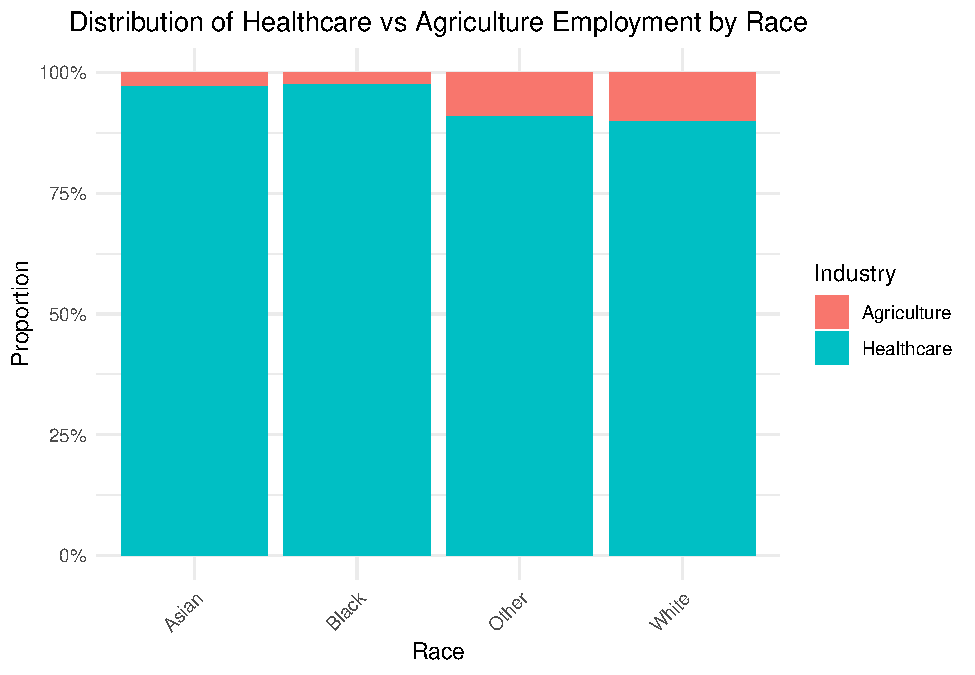
\includegraphics{nancee,-ummie-and-steven_files/figure-latex/unnamed-chunk-2-1.pdf}

\begin{Shaded}
\begin{Highlighting}[]
\CommentTok{\# Create regional distribution map}
\NormalTok{regional\_data }\OtherTok{\textless{}{-}}\NormalTok{ analyzed\_data }\SpecialCharTok{\%\textgreater{}\%}
  \FunctionTok{group\_by}\NormalTok{(region, industry) }\SpecialCharTok{\%\textgreater{}\%}
  \FunctionTok{summarise}\NormalTok{(}\AttributeTok{count =} \FunctionTok{n}\NormalTok{(), }\AttributeTok{.groups =} \StringTok{\textquotesingle{}drop\textquotesingle{}}\NormalTok{) }\SpecialCharTok{\%\textgreater{}\%}
  \FunctionTok{group\_by}\NormalTok{(region) }\SpecialCharTok{\%\textgreater{}\%}
  \FunctionTok{mutate}\NormalTok{(}\AttributeTok{proportion =}\NormalTok{ count}\SpecialCharTok{/}\FunctionTok{sum}\NormalTok{(count))}

\FunctionTok{ggplot}\NormalTok{(regional\_data, }\FunctionTok{aes}\NormalTok{(}\AttributeTok{x =}\NormalTok{ region, }\AttributeTok{y =}\NormalTok{ industry)) }\SpecialCharTok{+}
  \FunctionTok{geom\_tile}\NormalTok{(}\FunctionTok{aes}\NormalTok{(}\AttributeTok{fill =}\NormalTok{ proportion)) }\SpecialCharTok{+}
  \FunctionTok{scale\_fill\_viridis\_c}\NormalTok{(}\AttributeTok{labels =}\NormalTok{ scales}\SpecialCharTok{::}\NormalTok{percent) }\SpecialCharTok{+}
  \FunctionTok{theme\_minimal}\NormalTok{() }\SpecialCharTok{+}
  \FunctionTok{labs}\NormalTok{(}
    \AttributeTok{title =} \StringTok{"Industry Distribution Across Regions"}\NormalTok{,}
    \AttributeTok{x =} \StringTok{"Region"}\NormalTok{,}
    \AttributeTok{y =} \StringTok{"Industry"}\NormalTok{,}
    \AttributeTok{fill =} \StringTok{"Proportion"}
\NormalTok{  ) }\SpecialCharTok{+}
  \FunctionTok{theme}\NormalTok{(}
    \AttributeTok{axis.text.x =} \FunctionTok{element\_text}\NormalTok{(}\AttributeTok{angle =} \DecValTok{45}\NormalTok{, }\AttributeTok{hjust =} \DecValTok{1}\NormalTok{),}
    \AttributeTok{plot.title =} \FunctionTok{element\_text}\NormalTok{(}\AttributeTok{hjust =} \FloatTok{0.5}\NormalTok{)}
\NormalTok{  )}
\end{Highlighting}
\end{Shaded}

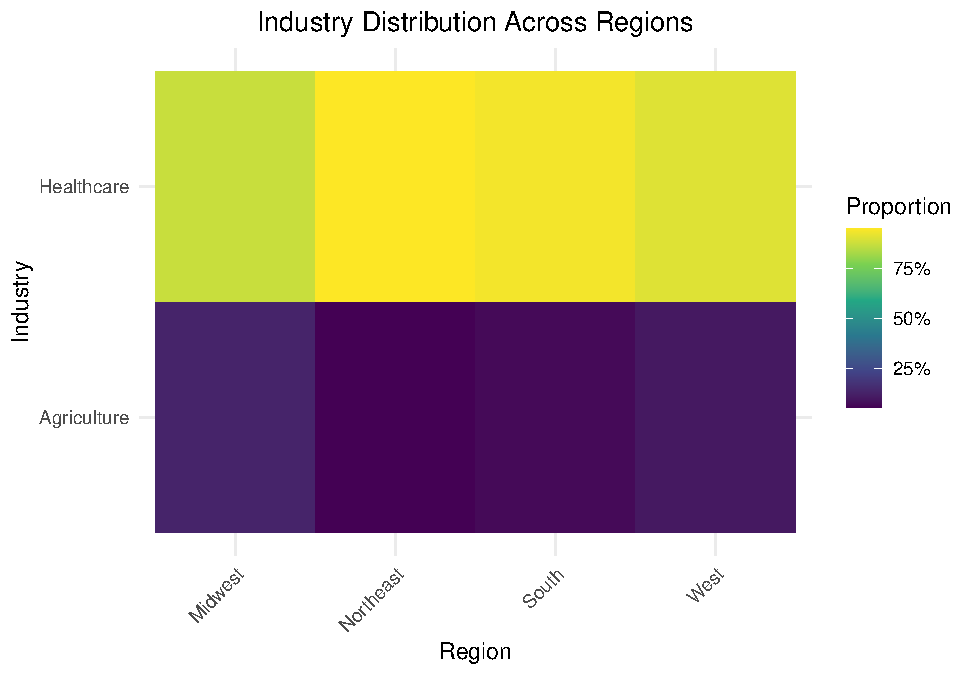
\includegraphics{nancee,-ummie-and-steven_files/figure-latex/unnamed-chunk-3-1.pdf}

\begin{Shaded}
\begin{Highlighting}[]
\CommentTok{\# Create contingency table}
\NormalTok{contingency\_table }\OtherTok{\textless{}{-}} \FunctionTok{table}\NormalTok{(analyzed\_data}\SpecialCharTok{$}\NormalTok{race, analyzed\_data}\SpecialCharTok{$}\NormalTok{industry)}

\CommentTok{\# Perform chi{-}square test}
\NormalTok{chi\_square\_test }\OtherTok{\textless{}{-}} \FunctionTok{chisq.test}\NormalTok{(contingency\_table)}

\CommentTok{\# Fisher\textquotesingle{}s exact test (for small sample sizes)}
\NormalTok{fisher\_test }\OtherTok{\textless{}{-}} \FunctionTok{fisher.test}\NormalTok{(contingency\_table, }\AttributeTok{simulate.p.value =} \ConstantTok{TRUE}\NormalTok{)}

\CommentTok{\# Create results table}
\NormalTok{test\_results }\OtherTok{\textless{}{-}} \FunctionTok{data.frame}\NormalTok{(}
  \AttributeTok{Test =} \FunctionTok{c}\NormalTok{(}\StringTok{"Chi{-}square"}\NormalTok{, }\StringTok{"Fisher\textquotesingle{}s Exact"}\NormalTok{),}
  \StringTok{"Statistic"} \OtherTok{=} \FunctionTok{c}\NormalTok{(chi\_square\_test}\SpecialCharTok{$}\NormalTok{statistic, }\ConstantTok{NA}\NormalTok{),}
  \StringTok{"p{-}value"} \OtherTok{=} \FunctionTok{c}\NormalTok{(chi\_square\_test}\SpecialCharTok{$}\NormalTok{p.value, fisher\_test}\SpecialCharTok{$}\NormalTok{p.value)}
\NormalTok{)}

\FunctionTok{kable}\NormalTok{(test\_results, }
      \AttributeTok{caption =} \StringTok{"Statistical Test Results"}\NormalTok{) }\SpecialCharTok{\%\textgreater{}\%}
  \FunctionTok{kable\_styling}\NormalTok{(}\AttributeTok{bootstrap\_options =} \FunctionTok{c}\NormalTok{(}\StringTok{"striped"}\NormalTok{, }\StringTok{"hover"}\NormalTok{))}
\end{Highlighting}
\end{Shaded}

\begin{longtable}[t]{llrr}
\caption{\label{tab:unnamed-chunk-4}Statistical Test Results}\\
\toprule
 & Test & Statistic & p.value\\
\midrule
X-squared & Chi-square & 788.0606 & 0.0000000\\
 & Fisher's Exact & NA & 0.0004998\\
\bottomrule
\end{longtable}

\begin{Shaded}
\begin{Highlighting}[]
\CommentTok{\# Calculate and display proportions}
\NormalTok{prop\_table }\OtherTok{\textless{}{-}} \FunctionTok{prop.table}\NormalTok{(contingency\_table, }\AttributeTok{margin =} \DecValTok{1}\NormalTok{) }\SpecialCharTok{*} \DecValTok{100}
\FunctionTok{kable}\NormalTok{(prop\_table, }
      \AttributeTok{caption =} \StringTok{"Industry Participation Rates by Race (\%)"}\NormalTok{) }\SpecialCharTok{\%\textgreater{}\%}
  \FunctionTok{kable\_styling}\NormalTok{(}\AttributeTok{bootstrap\_options =} \FunctionTok{c}\NormalTok{(}\StringTok{"striped"}\NormalTok{, }\StringTok{"hover"}\NormalTok{))}
\end{Highlighting}
\end{Shaded}

\begin{longtable}[t]{lrr}
\caption{\label{tab:unnamed-chunk-4}Industry Participation Rates by Race (%)}\\
\toprule
 & Agriculture & Healthcare\\
\midrule
Asian & 2.821870 & 97.17813\\
Black & 2.492212 & 97.50779\\
Other & 9.084821 & 90.91518\\
White & 10.153700 & 89.84630\\
\bottomrule
\end{longtable}

\begin{Shaded}
\begin{Highlighting}[]
\CommentTok{\# Test normality of employment distribution}
\NormalTok{employment\_counts }\OtherTok{\textless{}{-}}\NormalTok{ analyzed\_data }\SpecialCharTok{\%\textgreater{}\%}
  \FunctionTok{group\_by}\NormalTok{(race, industry) }\SpecialCharTok{\%\textgreater{}\%}
  \FunctionTok{summarise}\NormalTok{(}\AttributeTok{count =} \FunctionTok{n}\NormalTok{(), }\AttributeTok{.groups =} \StringTok{\textquotesingle{}drop\textquotesingle{}}\NormalTok{)}

\NormalTok{shapiro\_test }\OtherTok{\textless{}{-}} \FunctionTok{shapiro.test}\NormalTok{(employment\_counts}\SpecialCharTok{$}\NormalTok{count)}

\CommentTok{\# Create QQ plot}
\FunctionTok{ggplot}\NormalTok{(employment\_counts, }\FunctionTok{aes}\NormalTok{(}\AttributeTok{sample =}\NormalTok{ count)) }\SpecialCharTok{+}
  \FunctionTok{stat\_qq}\NormalTok{() }\SpecialCharTok{+}
  \FunctionTok{stat\_qq\_line}\NormalTok{() }\SpecialCharTok{+}
  \FunctionTok{theme\_minimal}\NormalTok{() }\SpecialCharTok{+}
  \FunctionTok{labs}\NormalTok{(}
    \AttributeTok{title =} \StringTok{"Q{-}Q Plot of Employment Counts"}\NormalTok{,}
    \AttributeTok{x =} \StringTok{"Theoretical Quantiles"}\NormalTok{,}
    \AttributeTok{y =} \StringTok{"Sample Quantiles"}
\NormalTok{  )}
\end{Highlighting}
\end{Shaded}

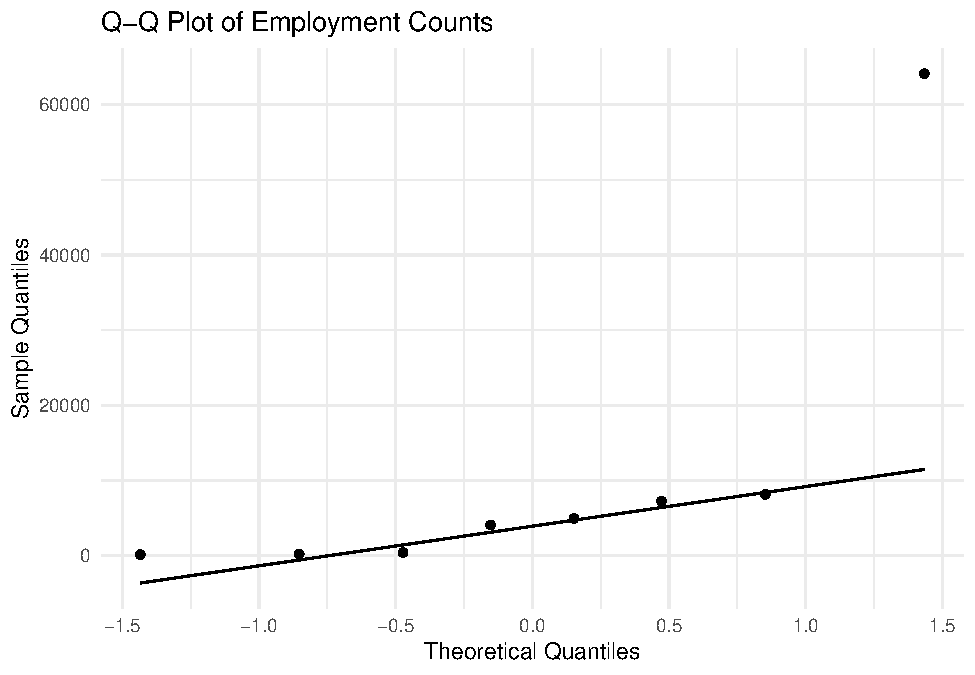
\includegraphics{nancee,-ummie-and-steven_files/figure-latex/unnamed-chunk-5-1.pdf}

You can also embed plots, for example:

Note that the \texttt{echo\ =\ FALSE} parameter was added to the code
chunk to prevent printing of the R code that generated the plot.

\end{document}
